\documentclass{article}
\usepackage[utf8]{inputenc}
\usepackage{amsmath, amssymb, physics, graphicx}
\usepackage{tikz}
\usepackage{caption}
\usetikzlibrary{arrows.meta, decorations.pathmorphing}

\title{Development of the Vorticity Equation in Duct Flows}

\begin{document}

\maketitle

\section{Introduction}

Vorticity is a key quantity in fluid dynamics, especially in complex flow geometries. This note analyzes the development and evolution of vorticity in two common situations: a curved duct (secondary vorticity generation) and an expanding duct (axial vorticity diffusion).

\vspace{1em}
We start from the Navier-Stokes equations for incompressible flow and derive the vorticity equation by applying the curl operator.

\section{Governing Equations}

\subsection{Navier-Stokes for Incompressible Flow}
\begin{equation}
    \frac{D\vec{u}}{Dt} = -\frac{1}{\rho}\nabla p + \nu \nabla^2 \vec{u}, \quad \text{with} \quad \nabla \cdot \vec{u} = 0
\end{equation}

\subsection{Vorticity Equation}
Taking the curl of the Navier-Stokes equations, we obtain:

\begin{equation}
    \frac{D\vec{\omega}}{Dt} = (\vec{\omega} \cdot \nabla)\vec{u} - (\vec{u} \cdot \nabla)\vec{\omega} + \nu \nabla^2 \vec{\omega}
\end{equation}

For incompressible flow, this simplifies to:

\begin{equation}
    \frac{D\vec{\omega}}{Dt} = (\vec{\omega} \cdot \nabla)\vec{u} + \nu \nabla^2 \vec{\omega}
\end{equation}

Where:

\begin{itemize}
    \item $(\vec{\omega} \cdot \nabla)\vec{u}$: Describes the stretching and tilting of vorticity. *Stretching* occurs when velocity gradients increase the magnitude of vorticity along its direction, while *tilting* refers to the reorientation of vorticity due to transverse velocity gradients.
    \item $\nu \nabla^2 \vec{\omega}$: Represents the viscous diffusion of vorticity, smoothing and spreading it out over time due to the fluid's viscosity.
\end{itemize}

\section{Case 1: 45° Curved Duct}

\begin{figure}[h!]*
    \centering
    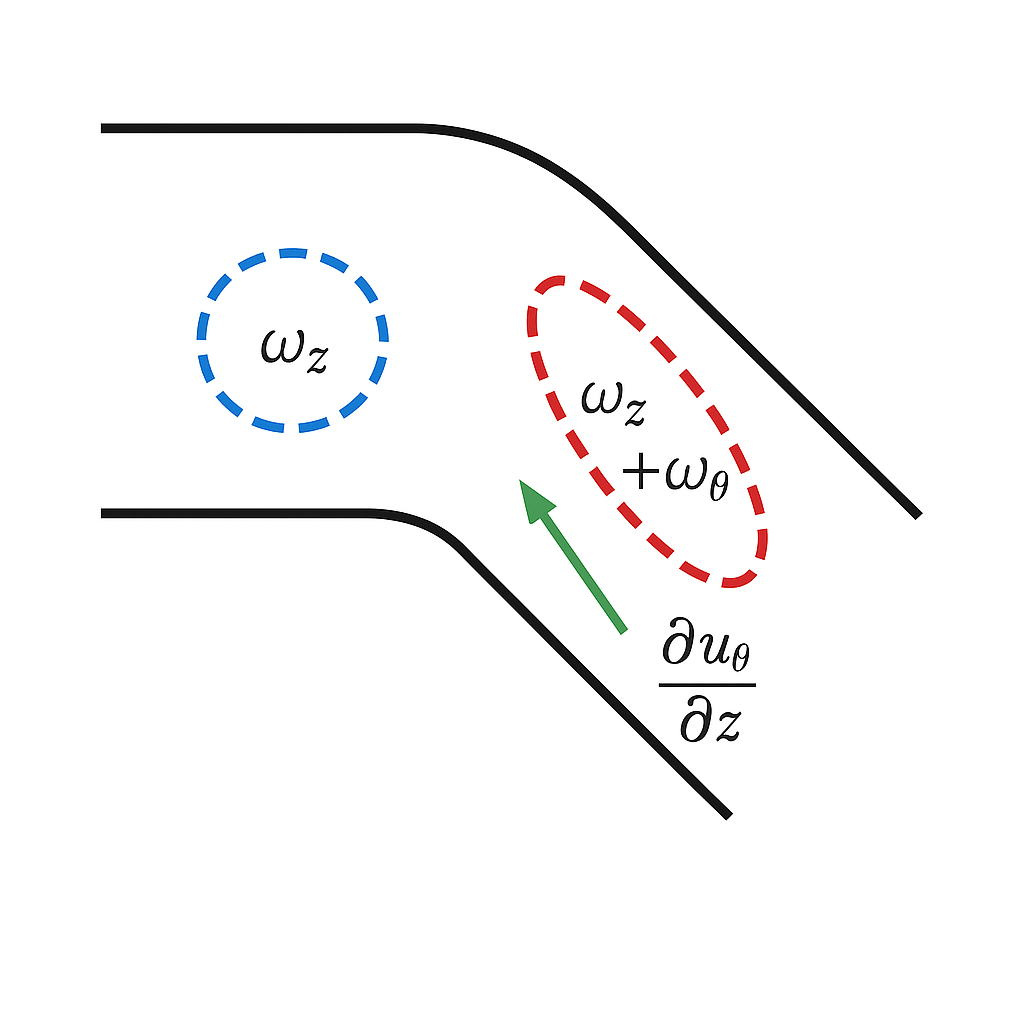
\includegraphics[width=0.6\textwidth]{vorticidad 45.png}
\end{figure}

\subsection{Assumptions}
\begin{itemize}
    \item Incompressible, laminar flow ($Re < 2300$)
    \item Newtonian fluid (shear stress proportional to velocity gradient, constant viscosity)
    \item Axial symmetry in the duct
    \item Smooth and steady curvature
    \item Negligible gravity effects
\end{itemize}

\subsection{Configuration}
Due to the duct's curvature, fluid particles near the outer wall must travel a longer path than those near the inner wall. To conserve flow rate, velocity increases near the outer wall and decreases near the inner wall, creating a velocity gradient.

\textbf{Dominant term:}
\[
(\vec{\omega} \cdot \nabla)\vec{u} \quad \text{(tilting and stretching)}
\]

\textbf{Justification:}
\begin{itemize}
    \item The curved path induces an azimuthal velocity component $u_\theta$ that varies in the axial ($z$) direction.
    \item This leads to a tilting/stretching effect:
    \[
    (\vec{\omega} \cdot \nabla)\vec{u} \approx \omega_z \frac{\partial u_\theta}{\partial z}
    \]
    \item Axial vorticity is converted into azimuthal vorticity, generating secondary flow structures (e.g., Dean vortices).
    \item While diffusion is present, it's secondary to the tilting/stretching effects.
\end{itemize}

\textbf{Conclusion:} In curved geometries, curvature induces stretching and tilting mechanisms that dominate vorticity evolution.

\subsection{Mathematical Development}
In cylindrical coordinates $(r,\theta,z)$, assuming initial axial vorticity $\omega_z$ dominates:

\begin{equation}
    (\vec{\omega} \cdot \nabla)\vec{u} = \omega_z \left(
        \frac{\partial u_r}{\partial z} \hat{e}_r +
        \frac{\partial u_\theta}{\partial z} \hat{e}_\theta +
        \frac{\partial u_z}{\partial z} \hat{e}_z
    \right)
\end{equation}

Since:
\[
\frac{\partial u_r}{\partial z} \ll \frac{\partial u_\theta}{\partial z}, \quad \frac{\partial u_z}{\partial z} \approx 0
\]

Then the dominant term is:
\begin{equation}
    (\vec{\omega} \cdot \nabla)\vec{u} \approx \omega_z \frac{\partial u_\theta}{\partial z} \hat{e}_\theta
\end{equation}

\subsection{Temporal Evolution of Vorticity}

Approximating the gradient as:
\begin{equation}
    \frac{\partial u_\theta}{\partial z} \approx \frac{\Omega \Delta r}{L_c}
\end{equation}

Then:
\begin{equation}
    \frac{D\omega_\theta}{Dt} \approx \omega_z \frac{\Omega \Delta r}{L_c} - \nu \left(\frac{\omega_\theta}{r^2}\right)
\end{equation}

\begin{itemize}
    \item \textbf{Initial state:} Vorticity mainly axial, forming a symmetric vortex ring.
    \item \textbf{Entering the curve:} $\partial u_\theta/\partial z$ becomes nonzero due to curvature.
    \item \textbf{Result:} Axial vorticity is tilted into the azimuthal direction, generating new vorticity component $\omega_\theta$.
    \item The vortex ring deforms, becoming elliptical and helicoidal, forming secondary vortices.
\end{itemize}

\textbf{Conclusion:} Curvature creates $\omega_\theta$ through stretching of axial vorticity, producing secondary vortex structures.

\section{Case 2: Expanding Duct}

\subsection{Assumptions}

\begin{center}
    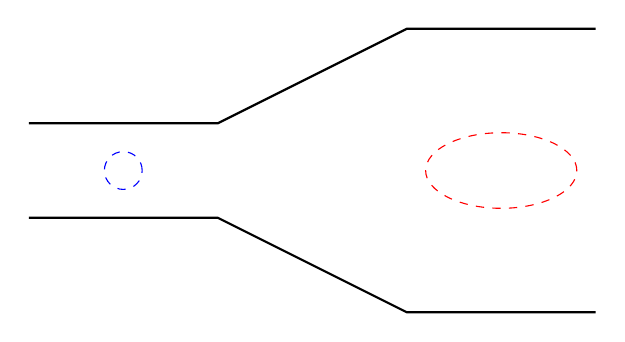
\begin{tikzpicture}[scale=1.2]
        \draw[thick] (0,-2) -- (2,-2) -- (4,-3) -- (6,-3);
        \draw[thick] (0,-1) -- (2,-1) -- (4,0) -- (6,0);
        \draw[dashed, blue] (1,-1.5) circle (0.2);
        \draw[dashed, red] (5,-1.5) ellipse (0.8 and 0.4);
    \end{tikzpicture}
\end{center}

\begin{itemize}
    \item Gradual expansion of cross-sectional area $A(z)$
    \item Flow rate conserved: $Q = A(z)u_z(z)$
    \item Initially axial vorticity: $\vec{\omega}(0) = \omega_0 \hat{e}_z$
    \item Incompressible, laminar flow
\end{itemize}

\textbf{Dominant term:}
\[
\nu \nabla^2 \vec{\omega} \quad \text{(viscous diffusion)}
\]

\textbf{Justification:}
\begin{itemize}
    \item No curvature or velocity gradients that would induce tilting or stretching.
    \item As the duct expands, axial velocity decreases, and no new vorticity is generated.
    \item Vorticity spreads radially due to viscosity:
    \[
    \frac{\partial \omega_z}{\partial t} \approx \nu \nabla^2 \omega_z
    \]
\end{itemize}

\textbf{Conclusion:} In expanding ducts, vorticity evolution is dominated by viscous diffusion in the absence of stretching or tilting mechanisms.

\subsection{Vorticity Evolution}

Simplified cylindrical form:

\begin{equation}
    \frac{\partial \omega_z}{\partial t} + u_z \frac{\partial \omega_z}{\partial z} = \frac{\nu}{r} \frac{\partial}{\partial r} \left( r \frac{\partial \omega_z}{\partial r} \right)
\end{equation}

\textit{Note:} $\nabla^2 = \frac{1}{r} \frac{\partial}{\partial r} \left( r \frac{\partial}{\partial r} \right) + \frac{1}{r^2} \frac{\partial^2}{\partial \theta^2}$

Self-similar solutions:

\begin{equation}
    \omega_z(r,t) = \frac{\Gamma_0}{4\pi \nu t} \exp\left(-\frac{r^2}{4\nu t}\right)
\end{equation}

\begin{equation}
    R(t) = \sqrt{R_0^2 + 4\nu t}
\end{equation}

\subsection{Circulation Conservation}
\begin{equation}
    \Gamma = \int_0^{R(z)} \omega_z \cdot 2\pi r \, dr = \Gamma_0 = \text{const}
\end{equation}

\begin{itemize}
    \item \textbf{Initial state:} Axial vorticity concentrated near the centerline.
    \item \textbf{Effect of expansion:} Larger cross-section reduces velocity, promoting radial vorticity diffusion.
    \item \textbf{Result:} The vortex ring spreads radially, peak vorticity drops, but total circulation is conserved.
\end{itemize}

\textbf{Conclusion:} Expansion causes axial vorticity to diffuse, broadening its profile while preserving total circulation.

\vspace{0.5cm}
\subsection*{General Comparison}

\begin{table}[h]
\centering
\begin{tabular}{|l|c|c|}
\hline
\textbf{Characteristic} & \textbf{Curved Duct} & \textbf{Expanding Duct} \\ \hline
Vortex ring deformation & Stretching + Tilting & Radial expansion \\ \hline
New vorticity components & Yes ($\omega_\theta \neq 0$) & No \\ \hline
Dominant mechanism & Tilting / Stretching & Viscous diffusion \\ \hline
Vorticity magnitude & May increase locally & Decreases globally \\ \hline
Total circulation & Conserved & Conserved \\ \hline
\end{tabular}
\caption{Comparison of vortex ring behavior}
\end{table}

\end{document}
